%
% LaTeX report template 
%

% This is a comment: in LaTeX everything that in a line comes
% after a "%" symbol is treated as comment

\documentclass[11pt, a4paper]{article}
\usepackage{graphicx}
\usepackage{amsmath}
\usepackage{listings}
\usepackage{url}
\usepackage{float}
\usepackage{xcolor}
\usepackage{hyperref}

\definecolor{codegreen}{rgb}{0,0.6,0}
\definecolor{codegray}{rgb}{0.5,0.5,0.5}
\definecolor{codepurple}{rgb}{0.58,0,0.82}
\definecolor{backcolour}{rgb}{0.95,0.95,0.92}
\definecolor{bg}{HTML}{212121}

\hypersetup{
  colorlinks=true,
  urlcolor=blue,
  linkcolor=blue,
  citecolor=blue,
}

% Define a command for the code output
\newcommand{\codeoutput}[1]{%
  \noindent\colorbox{bg}{%
    \begin{minipage}{\linewidth}%
      \textcolor{white}{\ttfamily #1}%
    \end{minipage}%
  }%
}

\lstdefinestyle{mystyle}{
    backgroundcolor=\color{backcolour},   
    commentstyle=\color{codegreen},
    keywordstyle=\color{magenta},
    numberstyle=\tiny\color{codegray},
    stringstyle=\color{codepurple},
    basicstyle=\ttfamily\footnotesize,
    breakatwhitespace=false,         
    breaklines=true,                 
    captionpos=b,                    
    keepspaces=true,                 
    numbers=left,                    
    numbersep=5pt,                  
    showspaces=false,                
    showstringspaces=false,
    showtabs=false,                  
    tabsize=2
}

\lstset{style=mystyle}

\title{EE5150: Communication Networks \\ Programming Assignment Report} % Title

\author{Ishaan Agarwal \\ EE20B046} % Author name

\date{\today} % Date for the report
\begin{document}		
		
\maketitle % Insert the title, author and date

\section{Introduction}
%Create new section;it is autonumbered
The aim of these problems is to simulate some fairly known concepts taught in the course and make observations in concurrence with theory taught in the lectures.


\section{The Geo/Geo/1 Queue}

We aim to simulate a discrete time Geo/Geo/1 queue i.e a discrete time queue with Bernoulli arrivals and services.
We start by defining the functions for arrivals and services in the following way:
\\

\begin{lstlisting}[language = Python]
def arrival(lamda):
    #This is a Bernoulli random variable with success probability lambda
    return np.random.choice([0,1], p=[1-lamda, lamda])

def service(mu):
    #This is a Bernoulli random variable with success probability mu
    return np.random.choice([0,1], p=[1-mu, mu])
\end{lstlisting}

\begin{figure}[H]
     \centering
     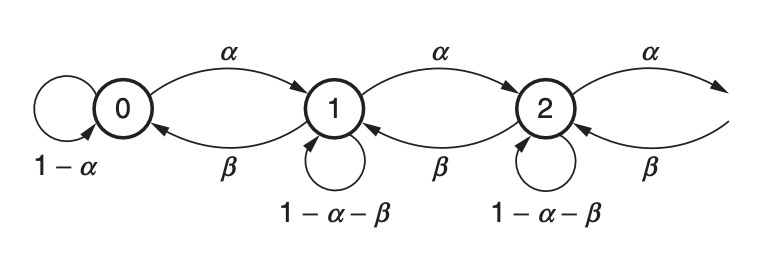
\includegraphics[scale=0.3]{Figure_1.png}
     \caption{The Discrete time Geo/Geo/1 Queue}
\end{figure}

\subsection{Simulating the Geo/Geo/1 Queue}
We simulate the queue for $T=10000$ time slots for $\lambda=0.1,0.2 \ldots 1$ for a constant $\mu = 0.9$. This is done in the following code block:
\\
\begin{lstlisting}[language = Python]
mu = 0.9
T = 10000 #total time
#queue length = number of packets in the queue at any time
#sojourn time = time spent in queue + time spent in service
lamda_range = np.arange(0.1, 1.1, 0.1)
average_q = []
average_sojourn_time = []

for lamda in lamda_range:
    ql = 0 #queue length
    q = [] #queue length at each time instant just before the arrival
    q.append(0)
    arrival_times = []
    service_times = []
    sojourn_times = []
    t = 1

    while t < T:
        if arrival(lamda):
            ql += 1
            arrival_times.append(t)
        if service(mu):
            if(ql!=0):
                ql-=1
                service_times.append(t)
        q.append(ql)
        t += 1

    average_q.append(np.mean(q))
    for i in range(len(service_times)): #computing only for those who have been served
        sojourn_times.append(service_times[i] - arrival_times[i])
    average_sojourn_time.append(np.mean(sojourn_times))

\end{lstlisting}


\subsection{Average Queue Lengths}
Now, we attempt to observe the average queue lengths versus the arrival rate $\lambda$. 
The corresponding code is:
\\
\begin{lstlisting}[language = Python]

print("Average values of queue length vs lamda:")
for i in range(1, len(average_q)+1):
    print("lamda = ", i/10, ":", average_q[i-1])

plt.plot(lamda_range, average_q, 'ro-')
plt.xlabel('lamda')
plt.ylabel('average queue length')
plt.grid()
plt.show()

\end{lstlisting}
The obtained output is as follows:
\begin{figure}[H]
     \centering
     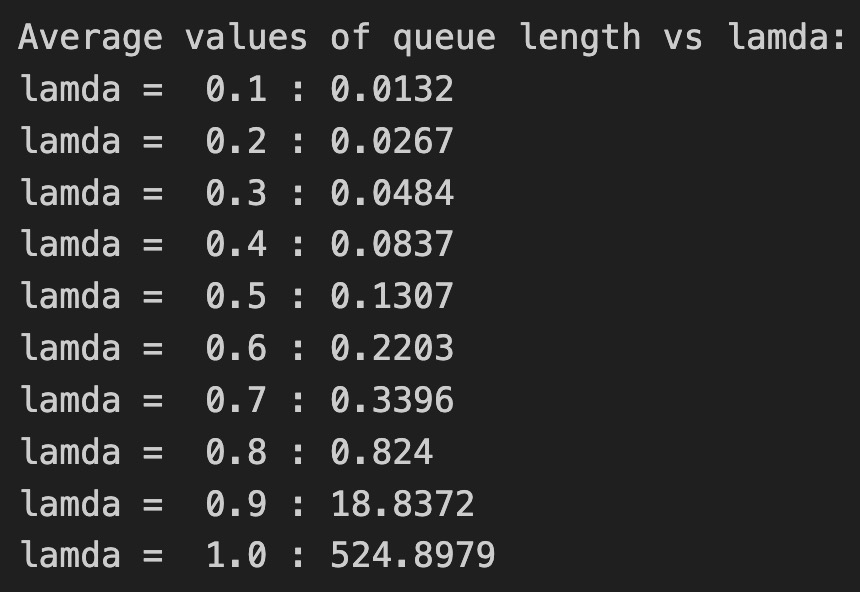
\includegraphics[scale=0.3]{Figure_4.png}
     \caption{Output}
\end{figure}

\begin{figure}[H]
     \centering
     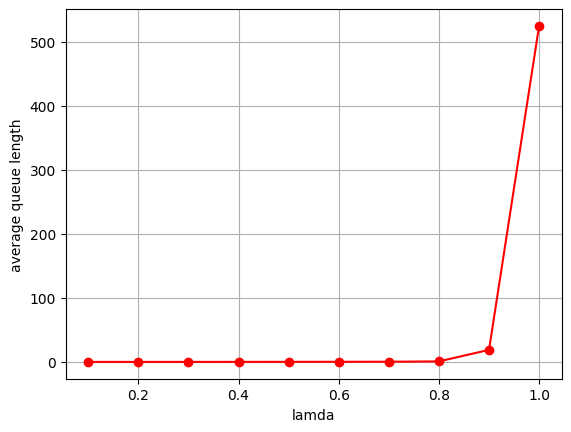
\includegraphics[scale=0.6]{Figure_2.png}
     \caption{Average queue lengths vs $\lambda$}
\end{figure}

We see that the average values of queue lengths are very small for $\lambda < 0.9$, this is because in these cases the arrivals are slower than services and thus, the queue length does not blow up, whereas in the other two cases, $\lambda \ge \mu$, and thus the queue length is significantly high.

\subsection{Simulations vs Theoretical}
In the previous part, we have observed the simulated queue length vs $\lambda$. In this part, let us compare that with the theoretical average queue lengths, which is computed by taking the expectation under a stationary distribution for the same set of parameters. 
\\
We know that for a finite state Geo/Geo/1 queue, the stationary distribution is given by the following (for max n customers in the system)(since infinite is not realisable on a machine, we take very large n value):
Local balance equations:
\[\pi(i)\lambda(1-\mu) = \pi(i+1)\mu(1-\lambda) \;\; \forall i = 0,1,2,\ldots,n-1\]
\[\implies \pi(i+1) = \pi(i)\rho \;\; \forall i = 0,1,2,...,n-1\]
\[\implies Pi(i) = \frac{(1-p)\rho^i}{(1-p^{(n+1)}}) \;\; \forall i = 0,1,2,...,n
\]
\[\rho = \frac{\lambda(1-\mu)}{\mu(1-\lambda)}\]
The codeblock for the following part is:
\begin{lstlisting}[language = Python]

#part (b):
n = 1000 #max queue length
mu = 0.9

theoretical_average_q = []

for lamda in lamda_range:
    p = lamda*(1-mu)/(mu*(1-lamda))
    Pi = np.zeros(n+1)
    #set Pi[0] = (1-p)(1-p**(n+1))
    Pi[0] = (1-p)/(1-p**(n+1))
    for i in range(1, n+1):
        Pi[i] = p**i*Pi[0]
    #Finding the expectation under the steady state distribution
    E = 0
    for i in range(n+1):
        E += i*Pi[i]
    theoretical_average_q.append(E)

print("Theoretical average queue length vs lamda:")
for i in range(1, len(theoretical_average_q)+1):
    print("lamda = ", i/10, ":", theoretical_average_q[i-1])

print("Simulated average queue length vs lamda:")
for i in range(1, len(average_q)+1):
    print("lamda = ", i/10, ":", average_q[i-1])

#plot theoretical average and simulated average on the same graph
plt.plot(lamda_range, theoretical_average_q, 'ro-', label='theoretical')
plt.plot(lamda_range, average_q, 'b--', label='simulated')
plt.xlabel('lamda')
plt.ylabel('average queue length')
plt.legend()
plt.grid()
plt.show()

\end{lstlisting}
The obtained output is:

\begin{figure}[H]
     \centering
     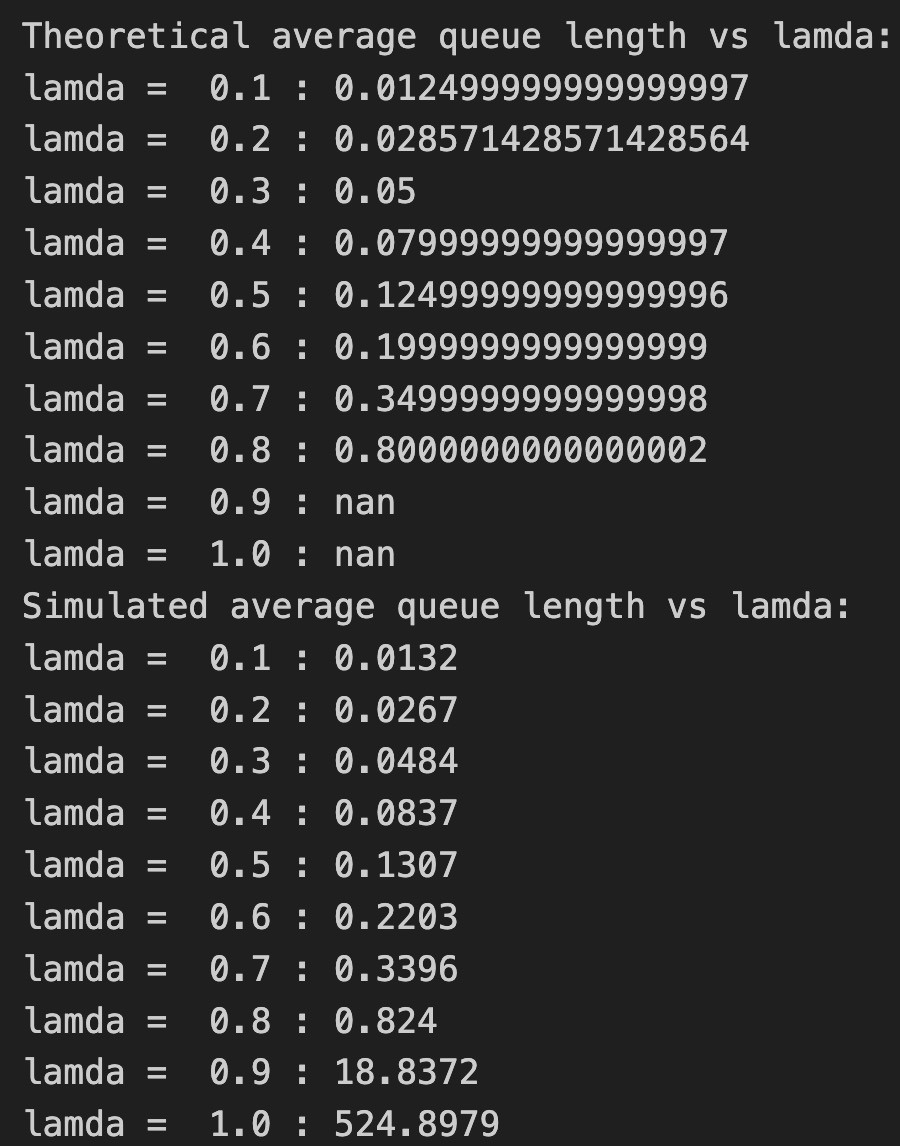
\includegraphics[scale=0.3]{Figure_6.png}
     \caption{Output}
\end{figure}
\begin{figure}[H]
     \centering
     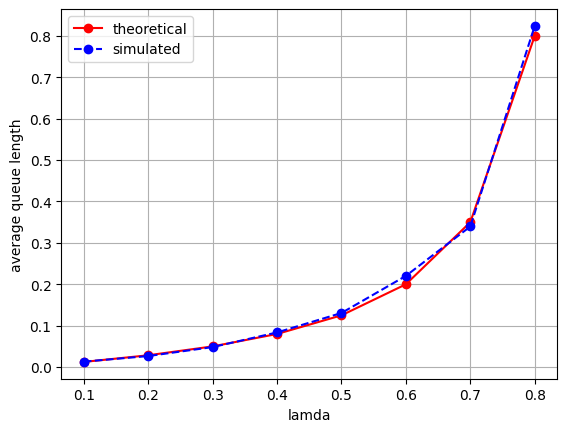
\includegraphics[scale=0.6]{Figure_7.png}
     \caption{Theoretical average queue lengths and Simulated Average Queue lengths vs $\lambda$}
\end{figure}

Note that the theoretical averages are not defined for $\lambda \ge 0.9$ because the sum of the geometric series only converges if $\lambda < \mu$, which is also our necessary condition for positive recurrence of the discrete time Markov chain corresponding to this process.

\subsection{Sojourn times}
Sojourn time is defined as the time from arrival till service completion of a packet, we want to observe the average sojourn times for each $\lambda$. This was done in the code block provided above by subtracting the arrival time from the service time for each packet and then taking the average. 
\\
\begin{lstlisting}[language = Python]
print("Average sojourn time vs lamda:")
for i in range(1, len(average_sojourn_time)+1):
    print("lamda = ", i/10, ":", average_sojourn_time[i-1])
plt.plot(lamda_range, average_sojourn_time, 'ro-')
plt.xlabel('lamda')
plt.ylabel('average sojourn time')
plt.grid()
plt.show()
\end{lstlisting}
The obtained output is as follows:
\begin{figure}[H]
     \centering
     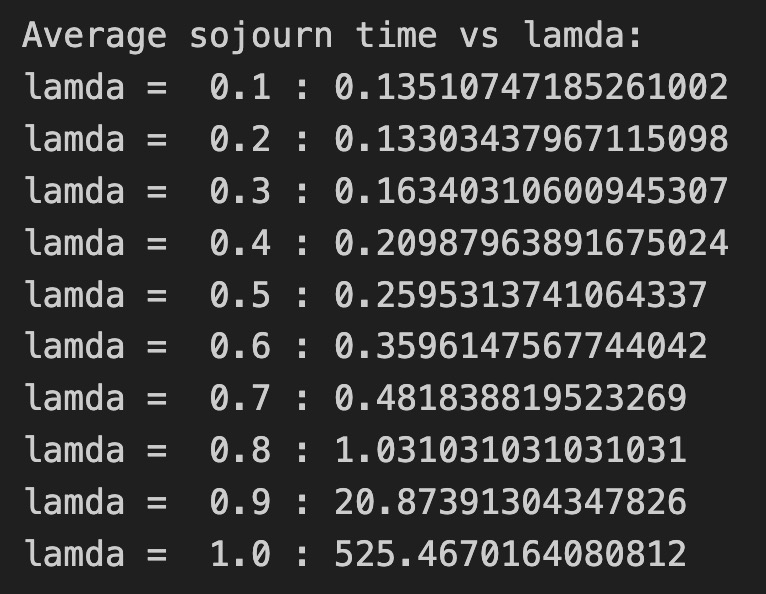
\includegraphics[scale=0.3]{Figure_3.png}
     \caption{Output}
\end{figure}
\begin{figure}[H]
     \centering
     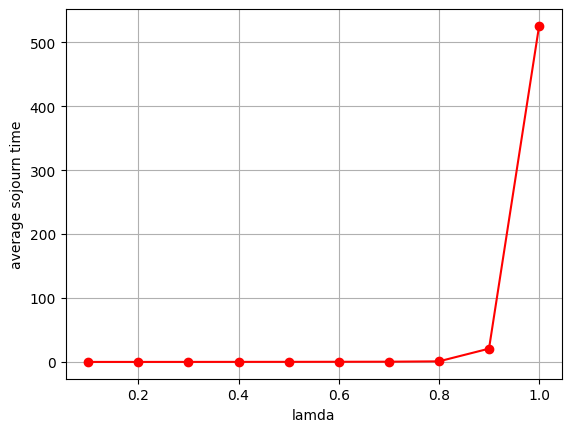
\includegraphics[scale=0.6]{Figure_5.png}
     \caption{Average sojourn times vs $\lambda$}
\end{figure}

\subsection{Little's Law}
Little's Law states that the average queue length is equal to the product of the mean arrival rate and the mean sojourn times. Let us verify this law from our simulations. 

\begin{lstlisting}[language = Python]
#Part c: Little's Theorem
#plotting the ration of average queue length and average sojourn time vs lamda
ratio = np.divide(average_q, average_sojourn_time)
print("Ratio of average queue length and average sojourn time vs lamda:")
for i in range(1, len(ratio)+1):
    print("lamda = ", i/10, ":", ratio[i-1])
plt.plot(lamda_range, ratio, 'ro--')
plt.xlabel('lamda')
plt.ylabel('ratio of average queue length and average sojourn time')
plt.grid()
plt.show()
\end{lstlisting}

Now, to verify that this ratio is indeed equal to the mean arrival rate, let us plot this ratio against $\lambda$, and then fit a least squares line to this using \texttt{np.linalg.lstsq} function.

\begin{lstlisting}[language = Python]
#Let us verify this by fitting a line to the plot
#We want to fit a least squares line to the data
#Fit a line y = mx + c to the data using numpy.linalg.lstsq
m, c = np.linalg.lstsq(np.vstack([lamda_range, np.ones(len(lamda_range))]).T, ratio, rcond = None)[0]
print("m = ", m, "c = ", c)
plt.plot(lamda_range, ratio, 'ro-', label='Original data', markersize=10)
plt.plot(lamda_range, m*lamda_range + c, 'b--', label='Fitted line')
plt.legend()
plt.grid()
plt.show()
#calculating mean squared error in percentage
mse = np.mean(np.square(np.subtract(ratio, m*lamda_range + c)))
print("Mean squared error in percentage = ", mse*100)
\end{lstlisting}

The graph obtained is as follows, with a slope of $m = 1.00394$ and an intercept of $c = -0.00067$, with a mean squared error of $0.001\%$ which shows that the obtained line is very close to the line $y=x$.


\begin{figure}[H]
     \centering
     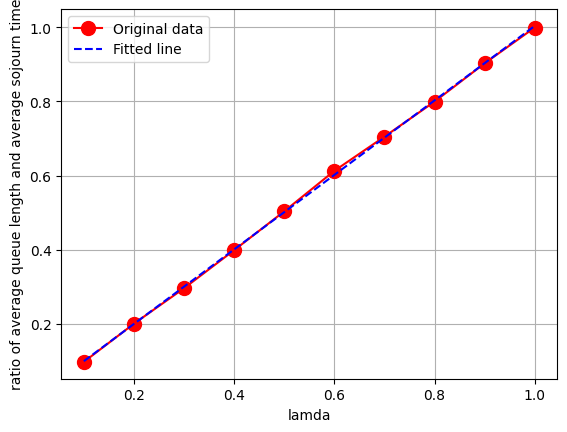
\includegraphics[scale=0.6]{Figure_8.png}
     \caption{Little's Law}
\end{figure}

\section{Conclusion}
We thus have simulated the discrete time Geo/Geo/1 queue and have verified the following results.
\begin{itemize}
\item Average queue lengths increase with arrival rate.
\item Average sojourn time increase with arrival rate.
\item The simulated average queue length was found to be very close to the theoretical average queue length.
\item Little's law was simulated and verified.
\end{itemize}

The code can be found here: \href{https://drive.google.com/drive/folders/1NdwyRu0YszZP-SYvFp2CQcfdz0ehORMg?usp=sharing}{Code}

\end{document}



 